\chapter{Evaluation}
\label{sec:evaluation}

\section{Approach \& On-path Velocity Constraint}

As expected, the $V_{approach}$ and $V_{path}$ is only expected in the Hybrid formulation.

\subsection{Low Speed On Path}

\includegraphics[width=0.7\textwidth]{VPath_0}

For a case where we desire to stop on the path, the hybrid formulation successfully demonstrates that it can approach the path orthogonally and come to a full stop.

\begin{figure}[h]
\centering
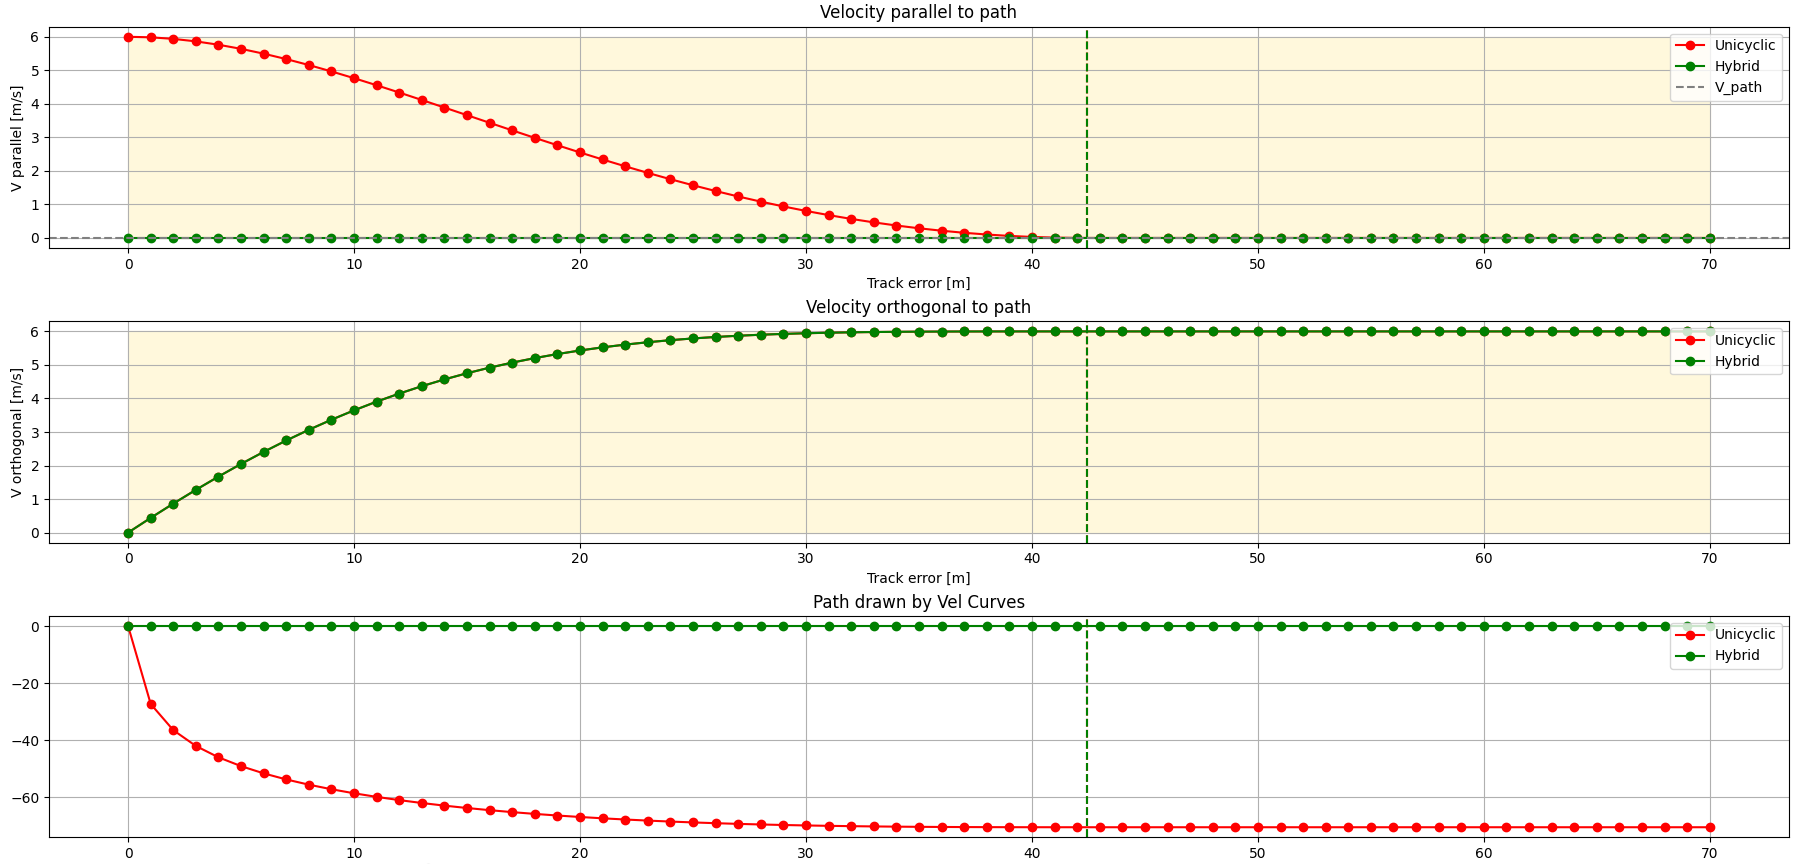
\includegraphics[width=\textwidth]{V_path_0_curve}
\caption{Velocity Curves with zero $V_{path}$}
\end{figure}

\subsection{High Speed On Path}

\includegraphics[width=0.7\textwidth]{VPath_High}

For a high speed on path case, hybrid formulation shows a different approach geometry.

\begin{figure}[h]
\centering
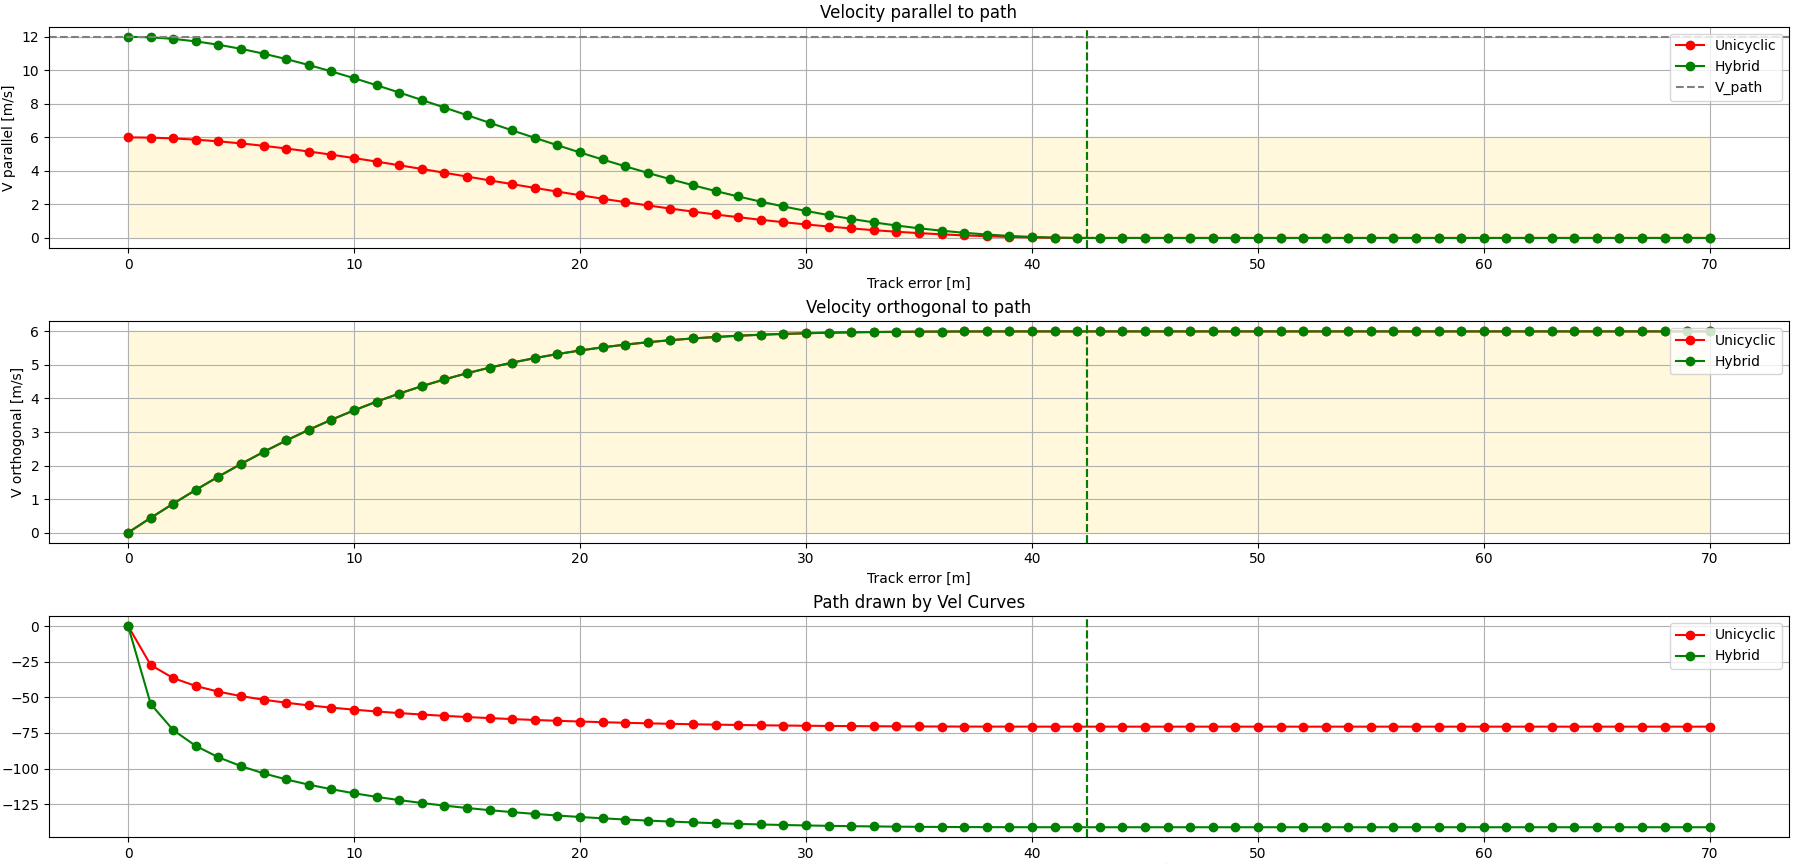
\includegraphics[width=\textwidth]{V_path_12_curve}
\caption{Velocity Curves with high $V_{path}$}
\end{figure}

\section{Acceleration Analysis}

\subsection{Path Orthogonal Acceleration}
The acceleration in the direction orthogonal to the path depends solely on the $V_{ref}^{\perp}(e)$ curve, and assuming vehicle perfectly following the reference velocity vector field, it can be calculated like following:

\begin{equation}
    \begin{split}
    \frac{d}{dt}V_{ref}^{\perp}(e) &= \frac{de}{dt}\frac{d}{de}V_{ref}^{\perp}(e)\\
    &= -V_{ref}^{\perp}(e) \cdot \frac{d}{de}V_{ref}^{\perp}(e)\\
    &= -V_{ref}^{\perp}(e) \cdot \frac{d\overline{e}}{de} \cdot \frac{d}{d\overline{e}}V_{ref}^{\perp}(\overline{e})\\
    &= V_{ref}^{\perp}(e) \cdot \frac{1}{e_b} \cdot V_{approach} \cdot sin(\theta_l(\overline{e})) \cdot \pi (\overline{e} - 1) \\
    &= \frac{V_{approach}^2}{e_b} \cdot \frac{sin(2\theta_l)}{2} \cdot \pi (\overline{e} - 1) \\
    &= \frac{\pi \cdot V_{approach}}{2t_{const}} \cdot sin(\pi (1-\overline{e})) \cdot (\overline{e} - 1)\\
    \end{split}
\label{eq:hybrid_orthogonal_acceleration_derive}
\end{equation}

\begin{figure}[h]
\centering
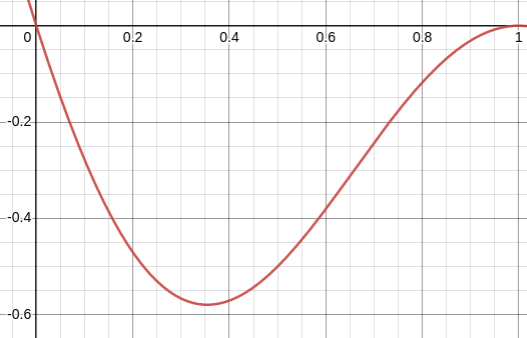
\includegraphics[width=0.6\textwidth]{Orthogonal_acceleration_desmos}
\label{eq:hybrid_orthogonal_acceleration_e_curve}
\end{figure}

Just take the right side of the final equation, this results in the following graph, which deterministically allows us to estimate the acceleration orthogonal to the path when following a track error boundary \autoref{eq:hybrid_track_error_boundary} and look ahead angle \autoref{eq:hybrid_quadratic_laa_curve} as multiplication of the $\frac{\pi \cdot V_{approach}}{2t_{const}}$ term and the graph.\\

And since by numerical analysis, the maximum negative acceleration occurs at $0.3542 \cdot e_b$, with a value of $-0.5792 \cdot \frac{\pi \cdot V_{approach}}{2t_{const}}$, the maximum magnitude of the orthogonal acceleration is determined as $0.9099 \cdot \frac{V_{approach}}{t_{const}}$.\\

Therefore, by picking a conservative value of $t_{const} = \frac{a_{max}^{mc}}{\sqrt{2} V_{approach}}$, the most aggressive approaching behavior can be chosen, which greatly improves the utilization of multirotor's agility compared to a unicyclic approach as demonstrated in the \autoref{tb:unicyclic_hybrid_a_max_comparison} below. Note, the $t_const$ for Unicyclic formulation was retrieved from the original paper\cite{stastny_flying_2019}, which was adapted for the fixed wing use case (thus, larger $t_{const}$).

\begin{table}[h]
\centering
\begin{tabular}{|c | c | c|}
 \hline
  & Unicyclic & Hybrid \\
 \hline
 $a_{max}^{mc} [m/s^2]$ & 10.0 & 10.0 \\ 
 \hline
$V_{approach / nom} [m/s]$ & 10.0 & 10.0 \\ 
 \hline
 $t_{const} [s]$ & 7.071 & 0.7071 \\ 
 \hline
 $a_{max}^{\perp} [m/s^2]$ & \textbf{0.643} & \textbf{6.434} \\
 \hline
\end{tabular}
\caption{Maximum Acceleration Utilized by Unicyclic vs Hybrid Formulation}
\label{tb:unicyclic_hybrid_a_max_comparison}
\end{table}

\section{Monotonicity Analysis}
Since the Velocity setpoint of the Hybrid Formulation\ref{eq:hybrid_velocity_components} is always a point on an ellipse, it is \textbf{guaranteed to be monotonic} as the look-ahead angle $\theta_l$ varies from 0 to $\frac{\pi}{2}$.

\section{Convergence Time Analysis}
Similarly to the acceleration analysis in \autoref{eq:hybrid_orthogonal_acceleration_derive}, convergence time also depends solely on the parameter $t_{const}$, since the absolute magnitude of the velocity was abstractified in \autoref{eq:hybrid_track_error_boundary}.\\

Therefore, since the hybrid formulation can utilize the acceleration constraint more flexibly (as shown in \autoref{tb:unicyclic_hybrid_a_max_comparison}), convergence time to the path is also always faster using the Hybrid formulation.

\section{Fixed Wing Case}

As shown below, the Hybrid formulation still encompasses the unicyclic formulation as a special case, when the $V_{path} = V_{approach}$, which is designated as $V_{nom}$.

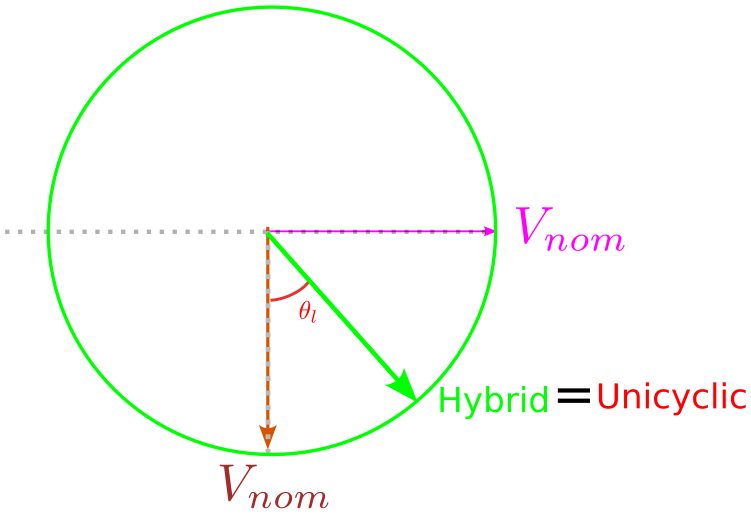
\includegraphics[width=0.7\textwidth]{Hybrid_Supporting_Unicyclic}